\documentclass{article}
\usepackage{graphicx}
\usepackage{tikz}
\usepackage{amsmath}
\usepackage{charter}
\usepackage{xcolor}
\usepackage[a4paper, margin=0.5in]{geometry}


\title{tikz Plots}
\author{FR }
\date{December 2024}

\begin{document}

\maketitle



\newpage

\section{Observational Unit Selection Criteria - Product Selection Strategies: An Overview}
\label{fig:selectcrit}
\begin{center}
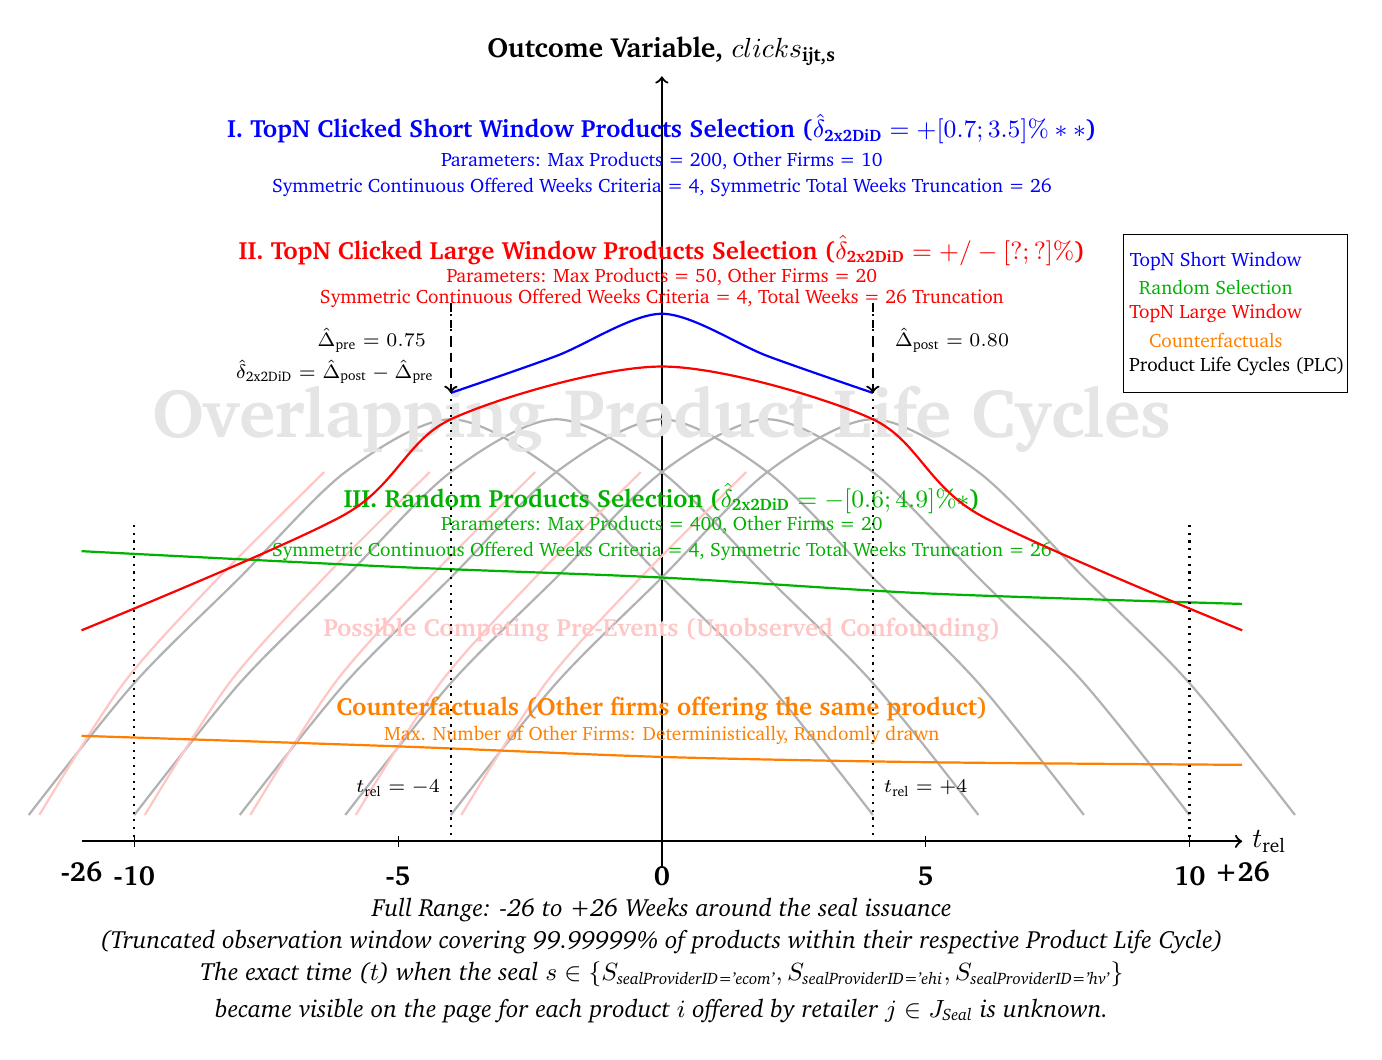
\begin{tikzpicture}[scale=0.67]

% Axes
\draw[->, thick] (-11,0) -- (11,0) node[right] {$t_\text{rel}$};
\draw[->, thick] (0,-0.5) -- (0,14.5) node[above] {\textbf{Outcome Variable, $clicks_\text{ijt,s}$}};

% Indicate Full Range of -26 to +26
\draw[dashed] (-10,0) -- (-11,0);
\draw[dashed] (10,0) -- (11,0);
\node[below] at (-11,-0.2) {\textbf{-26}};
\node[below] at (11,-0.2) {\textbf{+26}};
\node[below] at (0,-0.9) {\textit{\small Full Range: -26 to +26 Weeks around the seal issuance}};
\node[below] at (0,-1.5) {\textit{\small (Truncated observation window covering 99.99999\% of products within their respective Product Life Cycle)}};
\node[below] at (0,-2.1) {\textit{\small The exact time ($t$) when the seal $s \in \{S_\text{sealProviderID='ecom'}, S_\text{sealProviderID='ehi}, S_\text{sealProviderID='hv'}\}$}}; 
\node[below] at (0,-2.8) {\textit{\small became visible on the page for each product $i$ offered by retailer $j \in J_\text{Seal}$ is unknown.}};

% X-axis ticks and labels
\foreach \x in {-10, -5, 0, 5, 10} {
    \draw (\x,0.1) -- (\x,-0.1);
    \node[below] at (\x,-0.3) {\textbf{\x}};
}

% Overlapping Product Life Cycles (Background Annotation)
\node[gray!10] at (0,8) {\Huge \textbf{Overlapping Product Life Cycles}};

% Overlapping Product Life Cycles (Grey Curves)
\foreach \shift in {-4, -2, 0, 2, 4} {
    \draw[gray!60, thick] plot[smooth] coordinates {
        (-8+\shift,0.5) (-6+\shift,3) (-4+\shift,5) (-2+\shift,7) 
        (0+\shift,8) (2+\shift,7) (4+\shift,5) (6+\shift,3) (8+\shift,0.5)};
}

\node[gray!20] at (0,8) {\Huge \textbf{Overlapping Product Life Cycles}};

\node[pink!90] at (0,4) {\small \textbf{Possible Competing Pre-Events (Unobserved Confounding)}};

% Competing Events (Pink Curves)
\foreach \shift in {-4, -2, 0, 2, 4} {
    \draw[pink!90, thick] plot[smooth] coordinates {
        (-7.8+\shift,0.5) (-6.2+\shift,3) (-4.4+\shift,5) (-2.4+\shift,7)};
}

% TopN Short Window (blue curve)
\draw[blue, thick] plot[smooth] coordinates {
    (-4,8.5) (-2,9.2) (0,10) (2,9.2) (4,8.5)};
\node[blue] at (0,13.5) {\small \textbf{I. TopN Clicked Short Window Products Selection ($\hat{\delta}_{\text{2x2DiD}}=+[0.7;3.5]\%**$)}};
\node[blue] at (0,12.9) {\scriptsize Parameters: Max Products = 200, Other Firms = 10};
\node[blue] at (0,12.4) {\scriptsize Symmetric Continuous Offered Weeks Criteria = 4, Symmetric Total Weeks Truncation = 26};

% Random Product Selection (green line)
\draw[green!70!black, thick] plot[smooth] coordinates {
    (-11,5.5) (-5,5.2) (0,5) (5,4.7) (11,4.5)};
\node[green!70!black] at (0,6.5) {\small \textbf{III. Random Products Selection ($\hat{\delta}_{\text{2x2DiD}}=-[0.6;4.9]\%*$)}};
\node[green!70!black] at (0,6) {\scriptsize Parameters: Max Products = 400, Other Firms = 20};
\node[green!70!black] at (0,5.5) {\scriptsize Symmetric Continuous Offered Weeks Criteria = 4, Symmetric Total Weeks Truncation = 26};

% TopN Large Window (red curve)
\draw[red, thick] plot[smooth] coordinates {
    (-11,4.0) (-6,6.2) (-4,8) (0,9) (4,8) (6,6.2) (11,4.0)};
\node[red] at (0,11.2) {\small \textbf{II. TopN Clicked Large Window Products Selection ($\hat{\delta}_{\text{2x2DiD}}=+/-[?;?]\%$)}};
\node[red] at (0,10.7) {\scriptsize Parameters: Max Products = 50, Other Firms = 20};
\node[red] at (0,10.3) {\scriptsize Symmetric Continuous Offered Weeks Criteria = 4, Total Weeks = 26 Truncation};

% Counterfactuals (orange line)
\draw[orange, thick] plot[smooth] coordinates {
    (-11,2.0) (-5,1.8) (0,1.6) (5,1.5) (11,1.45)};
\node[orange] at (0,2.5) {\small 
\textbf{Counterfactuals (Other firms offering the same product)}};
\node[orange] at (0,2.0) {\scriptsize Max. Number of Other Firms: Deterministically, Randomly drawn};

% Mean Differences (Dotted Lines to Counterfactuals)
\draw[dotted, thick] (-4,10) -- (-4,0);
\draw[dotted, thick] (4,10) -- (4,0);
\draw[dotted, thick] (-10,6.0) -- (-10,0);
\draw[dotted, thick] (10,6.0) -- (10,0.0);

% Labels for Mean Differences
\node at (-5.0,1.0) {\scriptsize $t_\text{rel}=-4$};
\node at (5.0,1.0) {\scriptsize $t_\text{rel}=+4$};
% Rho Estimates (Example Estimates)
\draw[->, thick, dashed] (-4,10.2) -- (-4,8.5);
\node at (-5.5,9.5) {\scriptsize $\hat{\Delta}_{\text{pre}} = 0.75$};
\node at (-6.2,8.9) {\scriptsize $\hat{\delta}_{\text{2x2DiD}} = \hat{\Delta}_{\text{post}} - \hat{\Delta}_{\text{pre}}$};

\draw[->, thick, dashed] (4,10.2) -- (4,8.5);
\node at (5.5,9.5) {\scriptsize $\hat{\Delta}_{\text{post}} = 0.80$};

% Legend Box
\draw[fill=white] (8.75,8.5) rectangle (13.0,11.5);
\node[blue] at (10.5,11.0) {\scriptsize TopN Short Window};
\node[green!70!black] at (10.5,10.5) {\scriptsize Random Selection};
\node[red] at (10.5,10.0) {\scriptsize TopN Large Window};
\node[orange] at (10.5,9.5) {\scriptsize Counterfactuals};
\node[black] at (10.9,9.0) {\scriptsize Product Life Cycles (PLC)};

\end{tikzpicture}

\end{center}\noindent
An illustration of three different observation unit selection criteria—\textbf{\textcolor{black}{Product Selection Strategies}}—is presented above.

\begin{enumerate}
    \item \textbf{\textcolor{blue}{TopN Clicked Short Window Products Selection}}
    \begin{itemize}
        \item \textbf{\textcolor{blue}{Maximum Products:}} 200
        \item \textbf{\textcolor{blue}{Other Firms:}} 10
        \item \textbf{\textcolor{blue}{Symmetric Continuous Offered Weeks Criteria:}} 4
        \item \textbf{\textcolor{blue}{Symmetric Total Weeks Truncation:}} 26
    \end{itemize}
    \item \textbf{\textcolor{red}{TopN Clicked Large Window Products Selection (Currently Calculated)}}
    \begin{itemize}
        \item \textbf{\textcolor{red}{Maximum Products:}} 50
        \item \textbf{\textcolor{red}{Other Firms:}} 20
        \item \textbf{\textcolor{red}{Symmetric Continuous Offered Weeks Criteria:}} 4
        \item \textbf{\textcolor{red}{Symmetric Total Weeks Truncation:}} 26
    \end{itemize}
    \item \textbf{\textcolor{green!70!black}{Random Products Selection}}
    \begin{itemize}
        \item \textbf{\textcolor{green!70!black}{Maximum Products:}} 400
        \item \textbf{\textcolor{green!70!black}{Other Firms:}} 20
        \item \textbf{\textcolor{green!70!black}{Symmetric Continuous Offered Weeks Criteria:}} 4
        \item \textbf{\textcolor{green!70!black}{Symmetric Total Weeks Truncation:}} 26
    \end{itemize}
\end{enumerate}

\noindent
\textbf{\textcolor{orange}{Counterfactuals}} (Other firms offering the same product)

\begin{itemize}
    \item \textbf{\textcolor{orange}{Maximum Number of Other Firms:}} Deterministically, randomly drawn for dataset replication.
\end{itemize}

\noindent
\textit{\textcolor{black}{Note: The selection criteria involve choosing products based on click metrics within specified time windows, considering offerings from other firms (counterfactual selection), and applying symmetric truncation to the observation periods.}}


\end{document}
